\documentclass[12pt]{article}
\usepackage[margin=0.75in]{geometry}
\geometry{a4paper}
\usepackage[T1]{fontenc} % Support Icelandic Characters
\usepackage[utf8]{inputenc} % Support Icelandic Characters
\usepackage{graphicx} % Support for including images
\usepackage{hyperref} % Support for hyperlinks
\usepackage{wrapfig}

\usepackage{algorithm}
\usepackage{algorithmicx}
\usepackage{listings}
\usepackage{color}
\usepackage{siunitx}

\usepackage[svgnames]{xcolor}

\usepackage[spanish]{babel}
\usepackage[latin1]{inputenc}
\usepackage[usenames]{color}

\definecolor{mGreen}{rgb}{0,0.6,0}
\definecolor{mGray}{rgb}{0.5,0.5,0.5}
\definecolor{mPurple}{rgb}{0.58,0,0.82}
\definecolor{backgroundColour}{rgb}{0.95,0.95,0.92}

\usepackage{listings}             % Include the listings-package
\lstdefinestyle{CStyle}{
    backgroundcolor=\color{backgroundColour},   
    commentstyle=\color{mGreen},
    keywordstyle=\color{blue},
    numberstyle=\tiny\color{mGray},
    stringstyle=\color{red},
    basicstyle=\footnotesize,
    breakatwhitespace=false,         
    breaklines=true,                 
    captionpos=b,                    
    keepspaces=true,                 
    numbers=left,                    
    numbersep=5pt,                  
    showspaces=false,                
    showstringspaces=false,
    showtabs=false,                  
    tabsize=2,
    language=C
}


%------------------------------------------------------------------
% TITLE
%------------------------------------------------------------------

\title{
\centerline{
    
\includegraphics[width=75mm]{unsa.png}}
    \vspace{0.5 cm}
        Programación de Sistemas - Laboratorio - Grupo B
        \\
        \\
        \\
        \textbf{Práctica Laboratorio N8} 
        \large  
        \\
        %SC-T-718-ATSR,Automatic Speech Recognition, 2019-1 
        %\\ 
        \small Universidad Nacional de San Agustín - Escuela Profesional de Ingeniería de Sistemas, Arequipa, Perú 
  }

\author{
    Carlos Alberto Mestas Escarcena
    \\
    \texttt{cmestas@unsa.edu.pe}
}

\date{Julio 2020}

\begin{document}

\maketitle

El desarrollo de este informe se puede encontrar en el repositorio de \textcolor{blue}{
    \href{https://github.com/CarlosMestas/Programacion_de_Sistemas_Laboratorio_B_Carlos_Mestas_Practica8}{GitHub}}, durante el mismo se utilizó \textcolor{blue}{\href{https://lubuntu.net/}{Lubuntu}} que es una distribución de Linux ligera basada en Ubuntu, instalada esta en \textcolor{blue}{\href{https://www.virtualbox.org/}{Virtual Box}} que nos permite crear una máquina virtual para nuestro S.O.
    
%%%%%

\clearpage
\newpage

\section{Estudia la orden uptime}

\subsection{¿Cuánto tiempo lleva en marcha el sistema?}
   Se puede observar que el sistema lleva en marcha 38 minutos.

\begin{figure}[h]
    \centering
    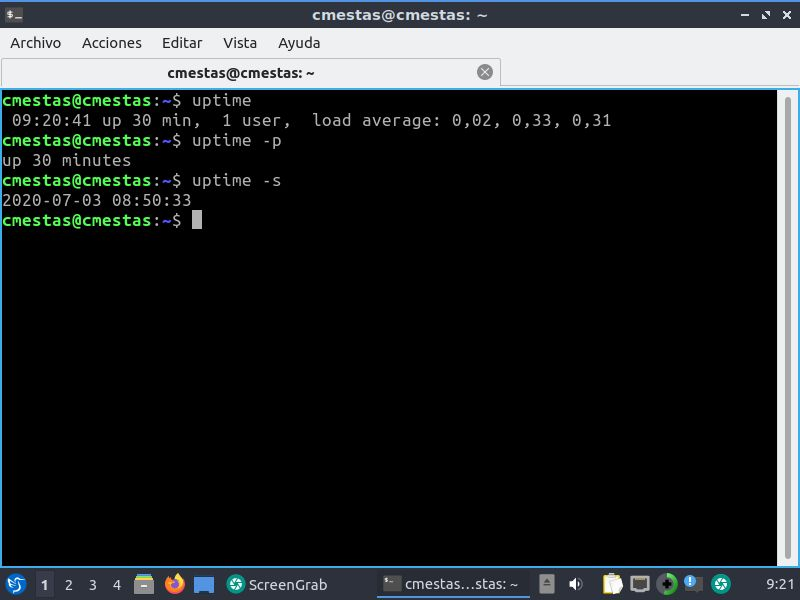
\includegraphics[width=1\textwidth]{images/screenA01.jpg}
    \caption{Comando $uptime$}
\end{figure}

Aparte de ello también podemos observar datos como:

\begin{itemize}
    \item La hora en la cual estamos realizando la consulta, en este caso $09:20:41$.
    \item Así como la cantidad de usuarios conectados en el momento, que solo es 1.
    \item Los promedios de carga del sistema de los últimos 1, 5 y 15 minutos que son 0.02, 0.33 y 0.31.
\end{itemize}

Si nosotros agregamos $-p$ al comando $uptime$ podemos solamente observar el tiempo en marcha del sistema, así como si agregamos $-s$ nos muestra la fecha y en la que comenzamos el uso del sistema.

\clearpage
\newpage

\subsection{¿Cuántos usuarios hay trabajando?}
Solamente tenemos un usuario trabajando actualmente.

\begin{figure}[h]
    \centering
    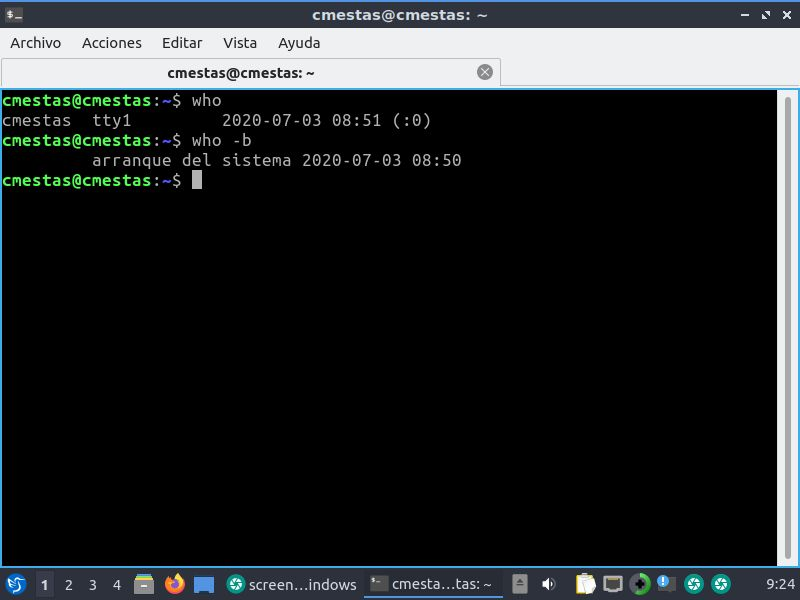
\includegraphics[width=1\textwidth]{images/screenA02.jpg}
    \caption{Comando $who$}
\end{figure}

Donde podemos observar que actualmente hay un usuario trabajando, así como la hora en la cual este se conectó.
Si le agregamos $-b$ al comando $who$ podemos observar solamente la fecha y hora en  la cual se inició el arranque del sistema.

\clearpage
\newpage

\subsection{¿Qué orden ofrece en su cabecera la misma información que uptime?}

\begin{figure}[h]
    \centering
    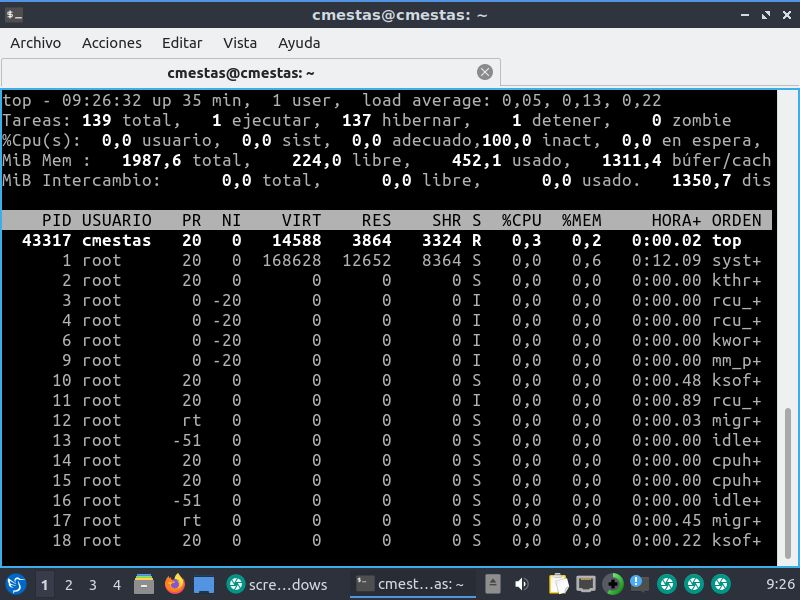
\includegraphics[width=0.8\textwidth]{images/screenA03.jpg}
    \caption{Comando $top$}
\end{figure}

El comando $top$ nos ofrece la misma información que $uptime$, cuando tiempo el sistema ya esta trabajando, la cantidad de usuarios actuales y los promedios de carga. Así como información extra.

\begin{figure}[h]
    \centering
    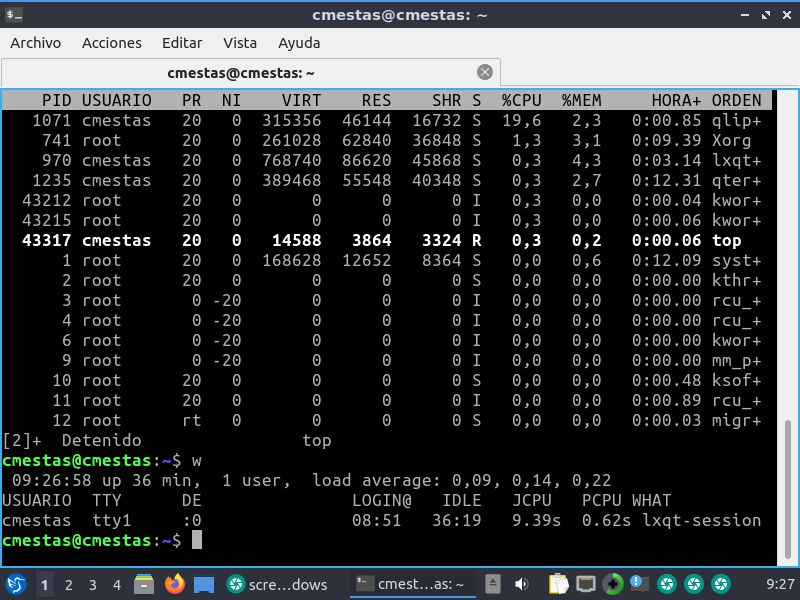
\includegraphics[width=0.5\textwidth]{images/screenA04.jpg}
    \caption{Comando $w$}
\end{figure}

También tenemos el comando $w$ que nos brinda también información del usuario, a que hora realizó el ingreso y otro datos como el tiempo que actualmente se encuentra.

\clearpage
\newpage

\section{La orden pstree muestra el árbol de procesos que hay en ejecución. Comprueba haciendo uso de la orden ps -la y de los valores “PID” y “PPID” mostrados para cada proceso, que efectivamente los procesos son padre e hijo.}

Si ejecutamos en segundo plano $(\#gedit~\&)$ un proceso, por ejemplo $gedit$, y hacemos un $ps~-la$:

\begin{figure}[h]
    \centering
    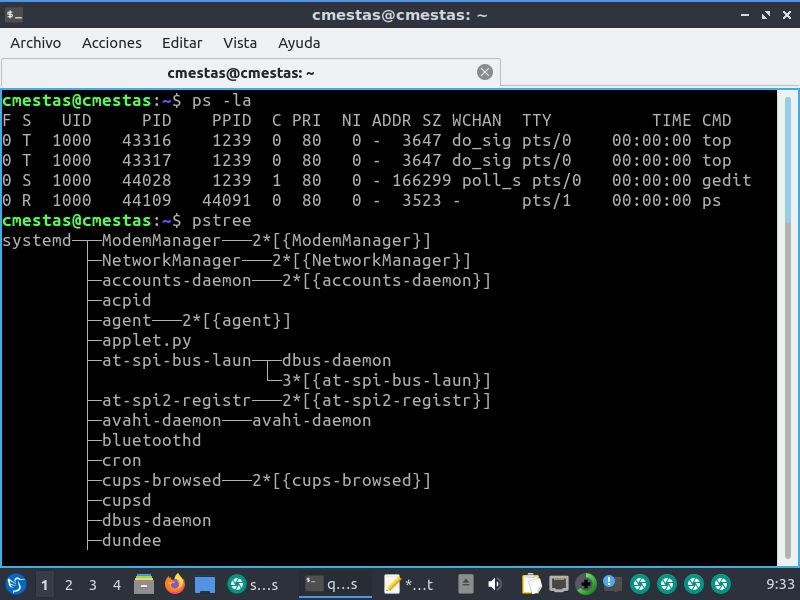
\includegraphics[width=0.6\textwidth]{images/screenA05.jpg}
    \caption{Comando $ps -la$}
\end{figure}

Observando que si tenemos el proceso $gedit$ con el $PPDI$ de $1239$.

\begin{figure}[h]
    \centering
    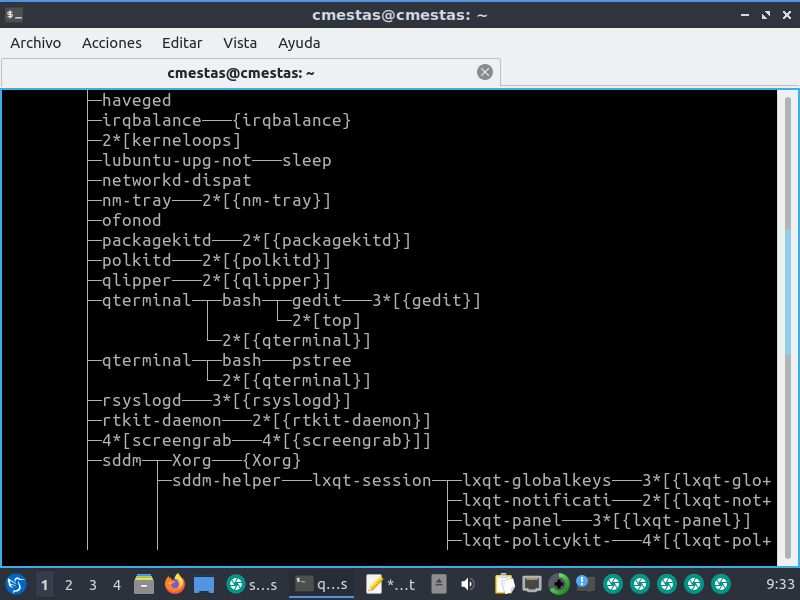
\includegraphics[width=0.6\textwidth]{images/screenA06.jpg}
    \caption{Comando $pstree$}
\end{figure}

Observamos que $gedit$ corresponde a $bash$.

\clearpage
\newpage

\section{En muchos casos nos interesará “cortar columnas”. Recuerda el uso de tr y cut. Por ejemplo, ¿cómo funciona esta instrucción?}

\begin{lstlisting}[language=bash,frame=single,style=CStyle]
ps aux | tr -s ' ' | cut -f 2,11 -d ' '
\end{lstlisting}

\begin{figure}[h]
    \centering
    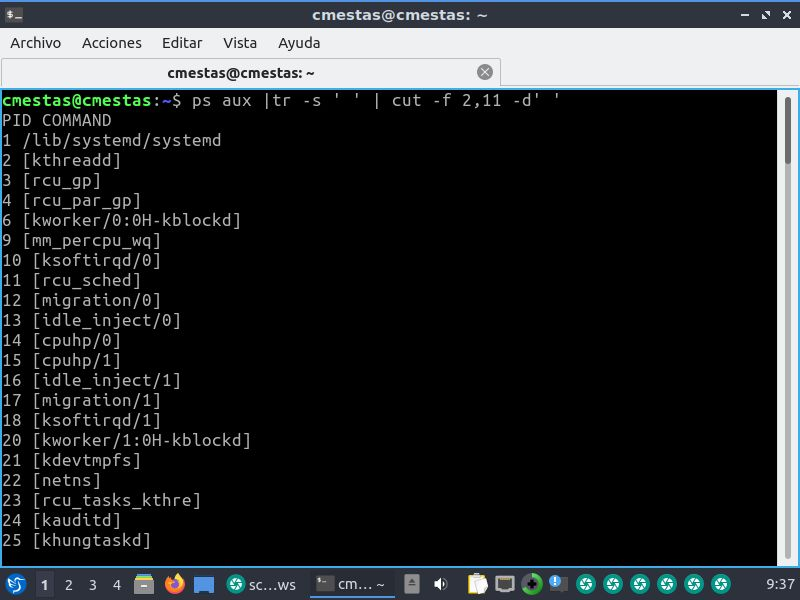
\includegraphics[width=1\textwidth]{images/screenA07.jpg}
    \caption{Comando \textit{ps aux} | \textit{tr -s} ' ' | \textit{cut -f 2,11} \textit{-d} ' '}
\end{figure}

\begin{itemize}
    \item \textbf{\textit{Ps aux}} lista los procesos de todos los usuarios.
    \item \textbf{\textit{Tr –s ' '}} elimina los espacios en blanco duplicados.
    \item \textbf{\textit{Cut –f 2,11 –d ' '}} corta por las columnas que nos interesa obtener información y usamos el delimitador.
\end{itemize}

\newpage
\clearpage

\section{Crea el fichero /tmp/bucle con el siguiente contenido}

\begin{lstlisting}[language=bash,frame=single,style=CStyle]
#!/bin/bash
echo ’nada’ > /dev/null 
exec /tmp/bucle
\end{lstlisting}

\begin{figure}[h]
    \centering
    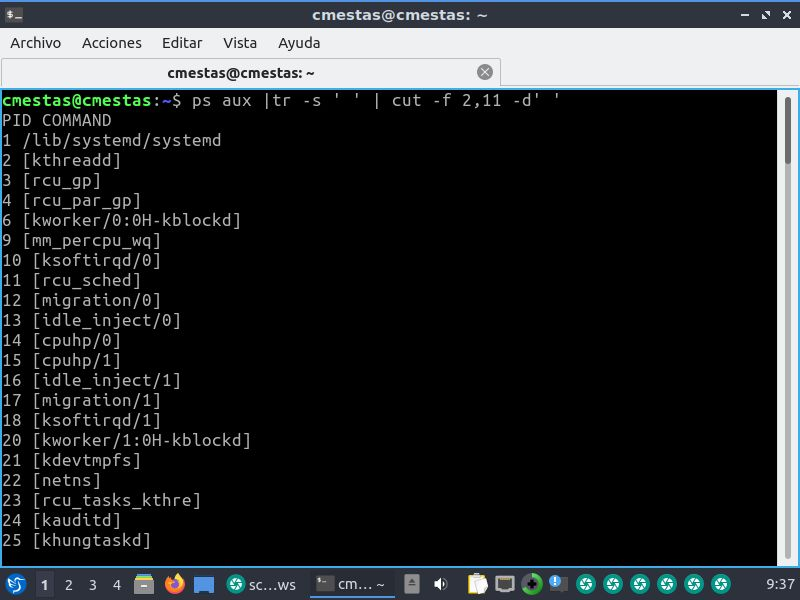
\includegraphics[width=1\textwidth]{images/screenA07.jpg}
    \caption{bucle}
\end{figure}

\begin{itemize}
    \item Ejecuta la orden $top$ en una terminal y comprueba el estado del sistema, a continuación lanza /tmp/bucle en otra. Observa cómo cambia el estado del sistema al lanzar el script. En una tercera terminal, comprueba con ps los procesos en ejecución.
\end{itemize}


\begin{figure}[h]
    \centering
    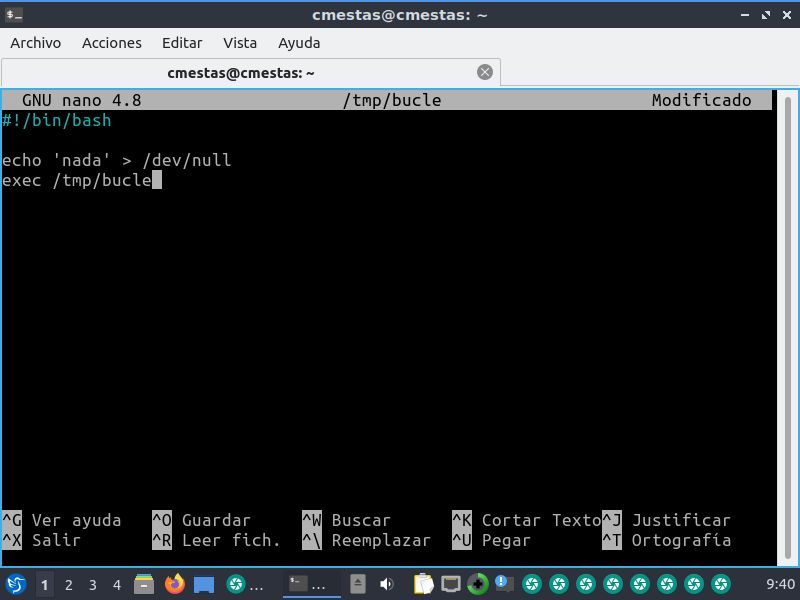
\includegraphics[width=0.7\textwidth]{images/screenA08.jpg}
    \caption{Editor nano: bucle}
\end{figure}

\begin{figure}[h]
    \centering
    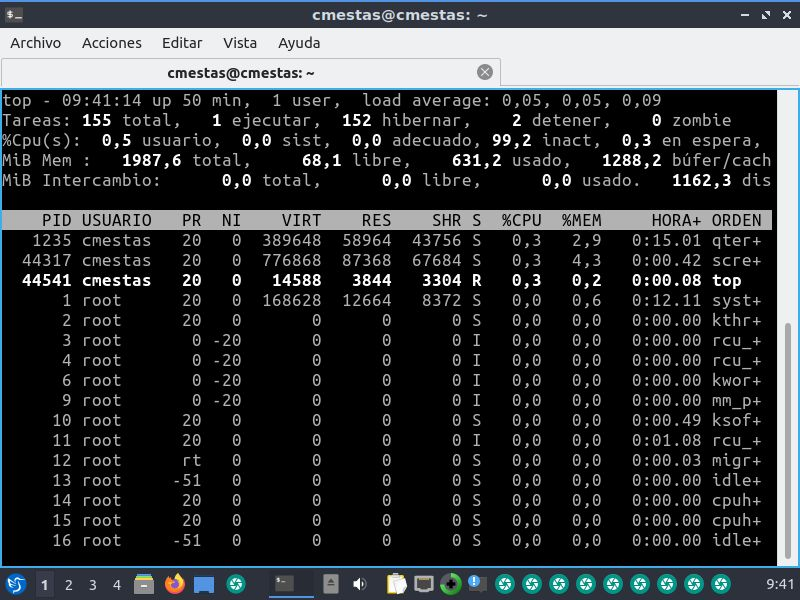
\includegraphics[width=0.7\textwidth]{images/screenA09.jpg}
    \caption{Antes de ejecutar el script}
\end{figure}

\clearpage
\newpage

\begin{figure}[h]
    \centering
    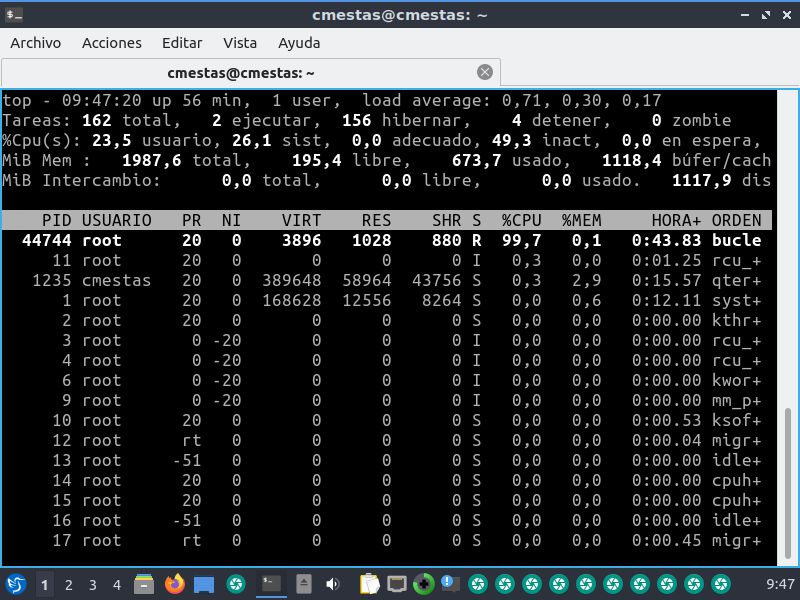
\includegraphics[width=0.7\textwidth]{images/screenA10.jpg}
    \caption{Luego de ejecutar el script}
\end{figure}

\begin{itemize}
    \item Usando la combinación de teclas “Control-Z” para el proceso bucle. Una vez parado comprueba que la información mostrada por $top$ va cambiando, hasta llegar un momento en el que no muestra información sobre dicho proceso. Fíjate que ha aumentado el número de procesos parados.
\end{itemize}

\begin{figure}[h]
    \centering
    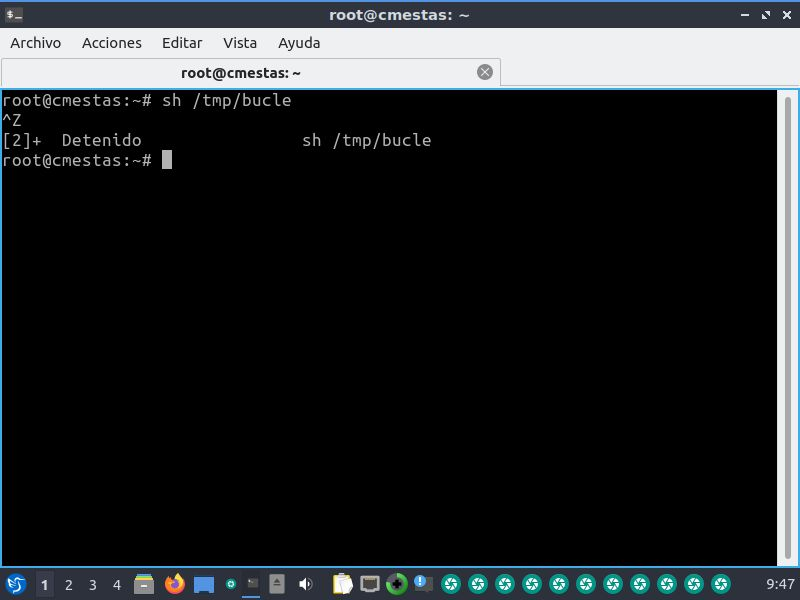
\includegraphics[width=0.6\textwidth]{images/screenA11.jpg}
    \caption{Ejecutando $``$Control - Z$"$ para detener el bucle}
\end{figure} 

\clearpage
\newpage

Observamos que tenemos un proceso detenido más, en comparación a los anteriores.

\begin{figure}[h]
    \centering
    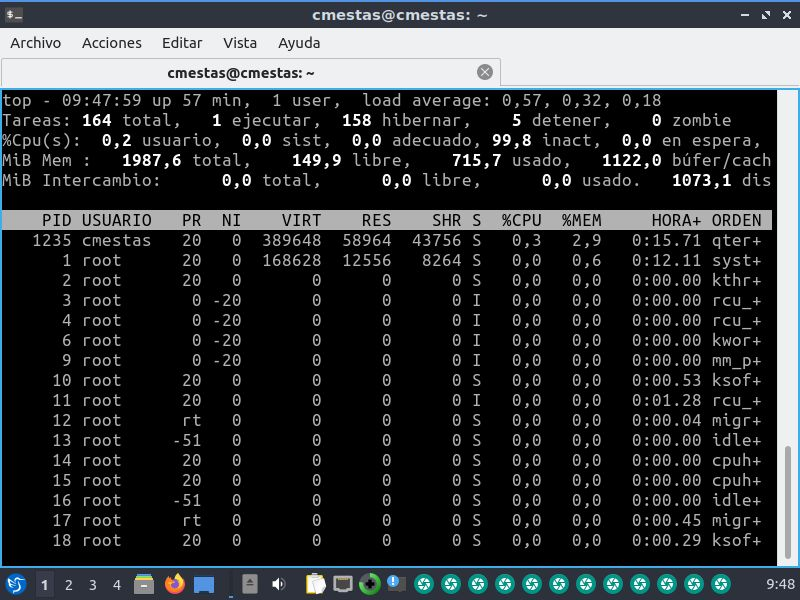
\includegraphics[width=0.7\textwidth]{images/screenA12.jpg}
    \caption{Comando $top$}
\end{figure}

\begin{itemize}
    \item Reinicia el proceso con la orden $fg$ y comprueba que vuelve a aparecer la información sobre el proceso.
\end{itemize}

\begin{figure}[h]
    \centering
    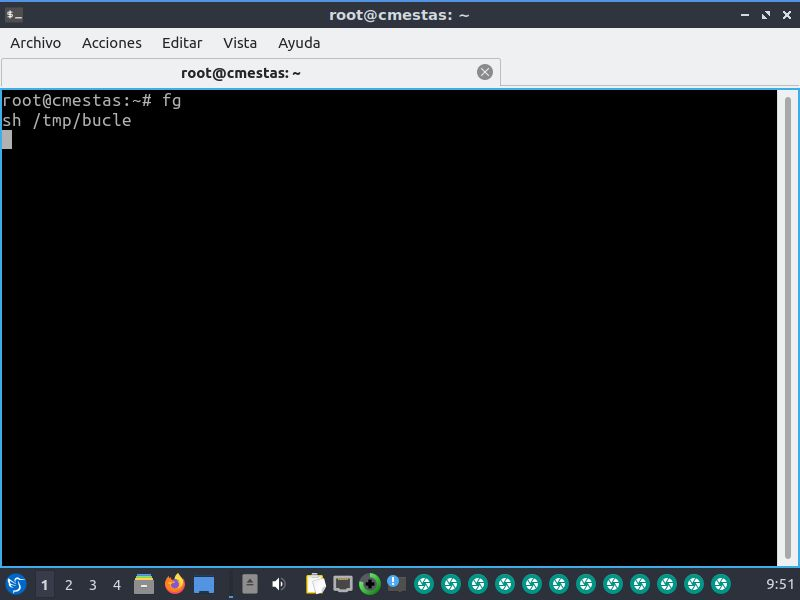
\includegraphics[width=0.6\textwidth]{images/screenA13.jpg}
    \caption{Comando $fg$}
\end{figure}

\clearpage
\newpage

El proceso vuelve a reanudarse.

\begin{figure}[h]
    \centering
    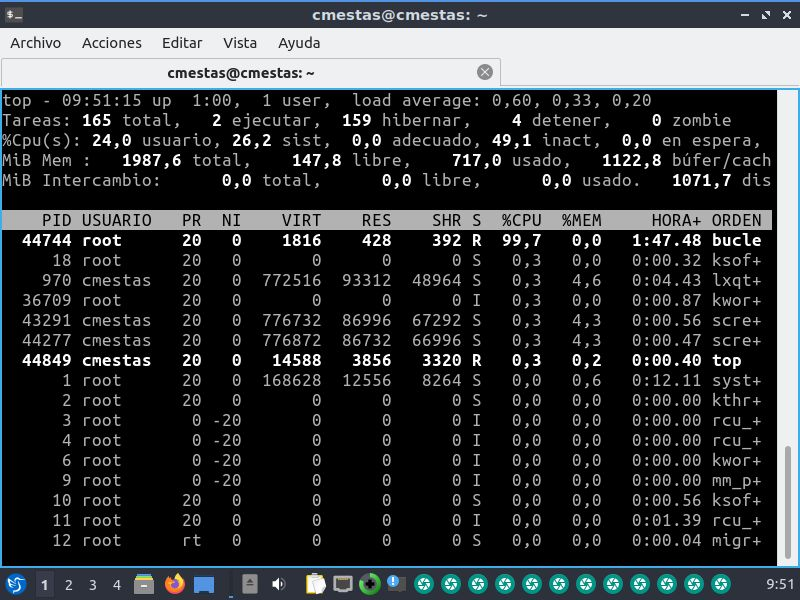
\includegraphics[width=1\textwidth]{images/screenA14.jpg}
    \caption{Comando $top$}
\end{figure}

\begin{itemize}
    \item Observa si mientras está en ejecución ese proceso cambia la carga media del sistema.
    \\
    \\
    Aumenta debido a que ejecutamos un bucle infinito.
    \item ¿Por qué aparece siempre el proceso bucle con el mismo $PID$ si se lanza a sí mismo una y otra vez durante su ejecución?
    \\
    \\
    Porque lo que realizamos con la combinación de teclas “Control-Z” durante la ejecución del script lo único que hace es pausar su ejecución, pero esta ejecución no termina, por lo cual el $PID$ no llega a cambiar, porque es el mismo proceso.
    \clearpage
    \newpage
    \item Cambia la velocidad de refresco de $top$ a 2s.
\end{itemize}

\begin{figure}[h]
    \centering
    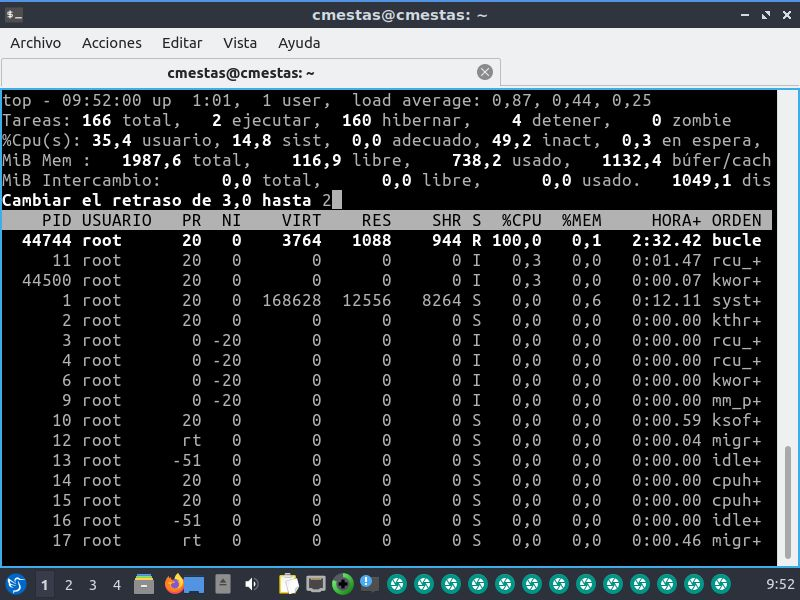
\includegraphics[width=0.7\textwidth]{images/screenA15.jpg}
    \caption{Comando $top$ cambiando la velocidad de refresco}
\end{figure}

\begin{itemize}
    \item Desde el top, cambia la prioridad del proceso, dándole un valor menor, por ejemplo 10.
\end{itemize}

\begin{figure}[h]
    \centering
    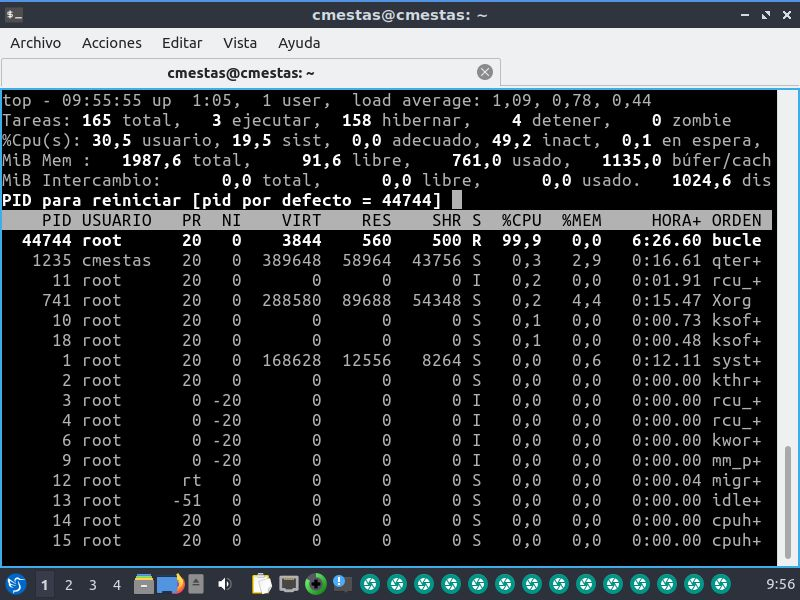
\includegraphics[width=0.6\textwidth]{images/screenA18.jpg}
    \caption{Comando $top$ cambiando la prioridad del proceso}
\end{figure}

\clearpage
\newpage

\begin{figure}[h]
    \centering
    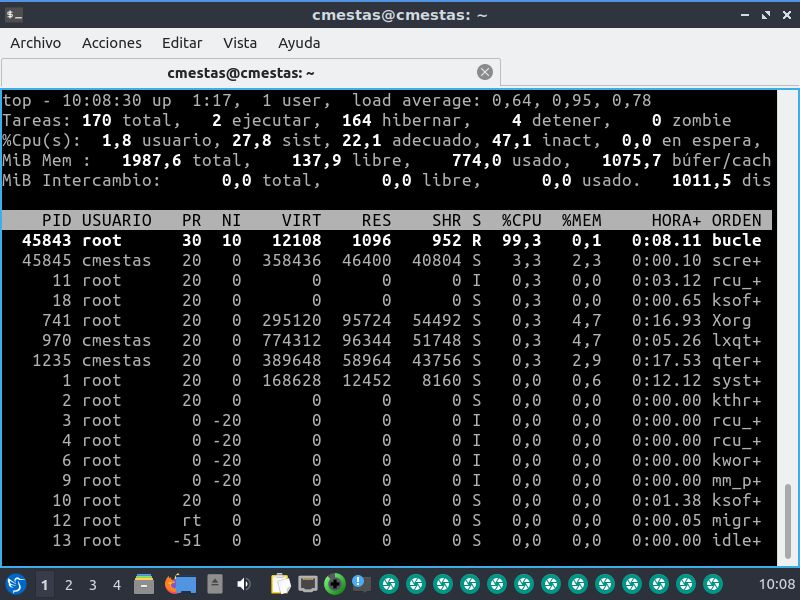
\includegraphics[width=0.65\textwidth]{images/screenA20.jpg}
    \caption{Comando $top$ luego del cambio de la prioridad}
\end{figure}

\begin{itemize}
    \item Usando la orden $nice$ lanza otro proceso bucle con la prioridad de 5.
\end{itemize}

\begin{figure}[h]
    \centering
    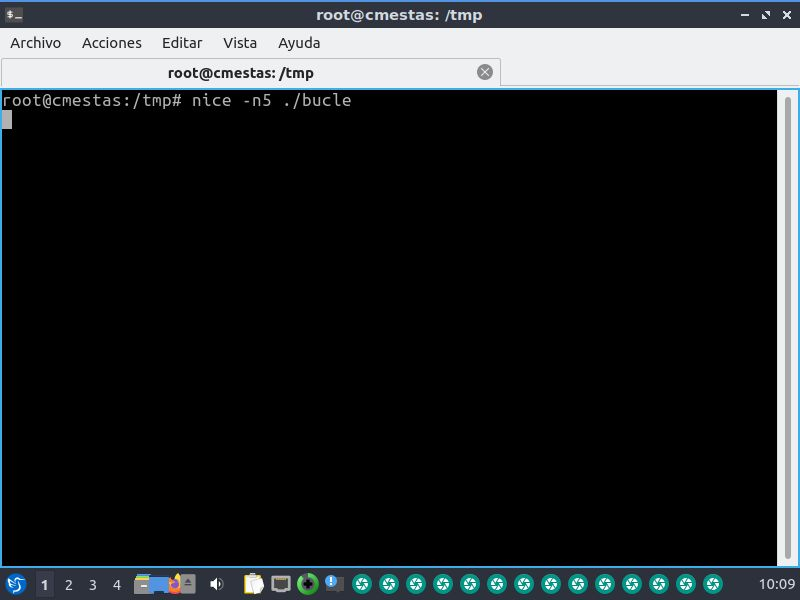
\includegraphics[width=0.65\textwidth]{images/screenA21.jpg}
    \caption{Agregamos otro bucle con prioridad de 5}
\end{figure}

\clearpage
\newpage

\begin{figure}[h]
    \centering
    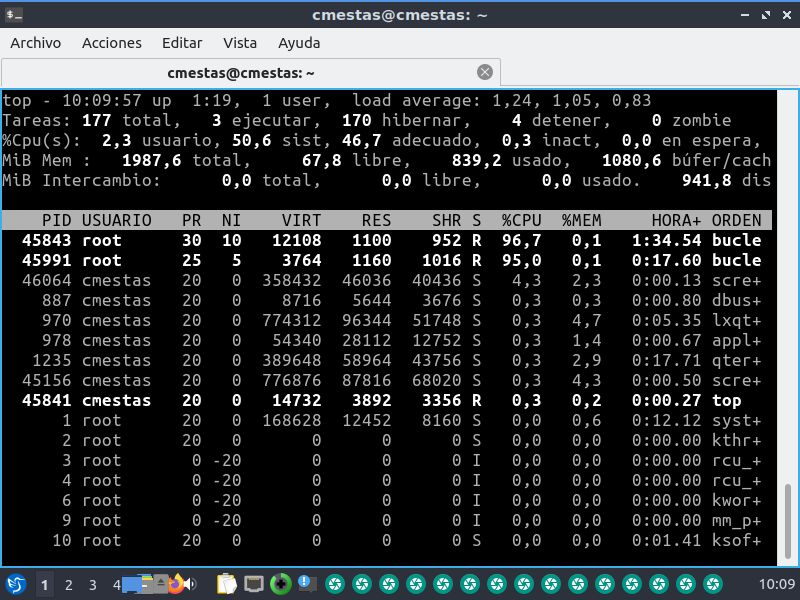
\includegraphics[width=0.65\textwidth]{images/screenA22.jpg}
    \caption{Ejecución de los dos bucles}
\end{figure}

\begin{itemize}
    \item Asigna mediante $renice$ una prioridad de 19 al bucle que lanzaste con prioridad 5. ¿Cómo afecta esto a la ejecución de los dos procesos?
\end{itemize}

\begin{figure}[h]
    \centering
    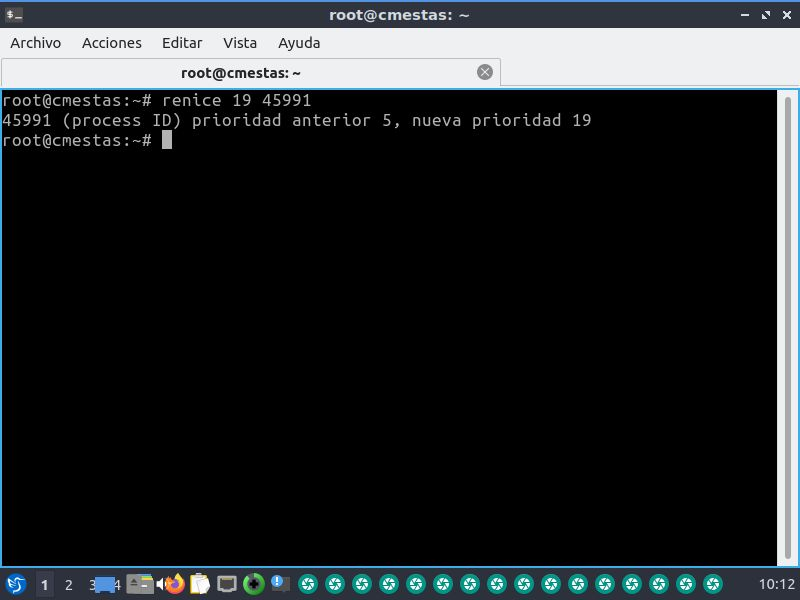
\includegraphics[width=0.65\textwidth]{images/screenA23.jpg}
    \caption{Cambio en la prioridad}
\end{figure}

Se puede observar un cambio cuando ejecutamos $top$.

\clearpage
\newpage

\begin{itemize}
    \item Desde el $top$ mata el bucle con prioridad 10. Fíjate que ahora, a pesar de que el que queda tiene prioridad 19, se le asigna más de la CPU que antes.
\end{itemize}

\begin{figure}[h]
    \centering
    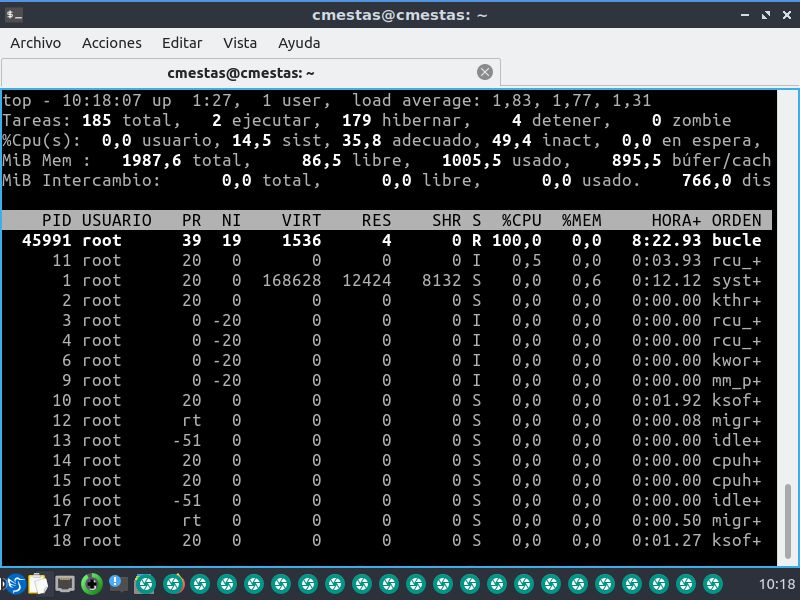
\includegraphics[width=0.65\textwidth]{images/screenA29.jpg}
    \caption{Luego de eliminar el que tenía prioridad 19}
\end{figure}

Ahora el otro proceso que queda ahora esta con el $\%100$ del uso del CPU.

\begin{itemize}
    \item Haciendo uso de la orden $kill$, para el proceso bucle que aún queda en ejecución. Después, usando también $kill$ reanúdalo y, finalmente, elimínalo.
\end{itemize}

\begin{figure}[h]
    \centering
    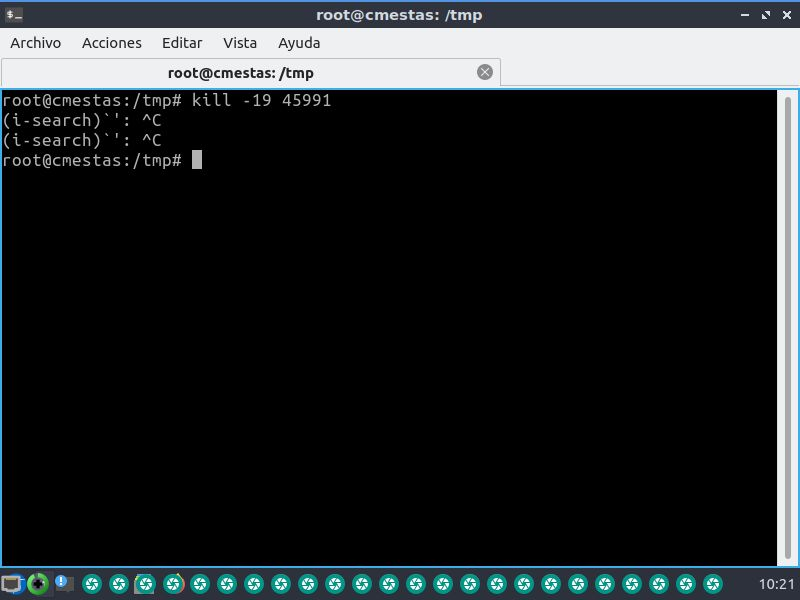
\includegraphics[width=0.65\textwidth]{images/screenA30.jpg}
    \caption{Pausamos el bucle}
\end{figure}

\begin{figure}[h]
    \centering
    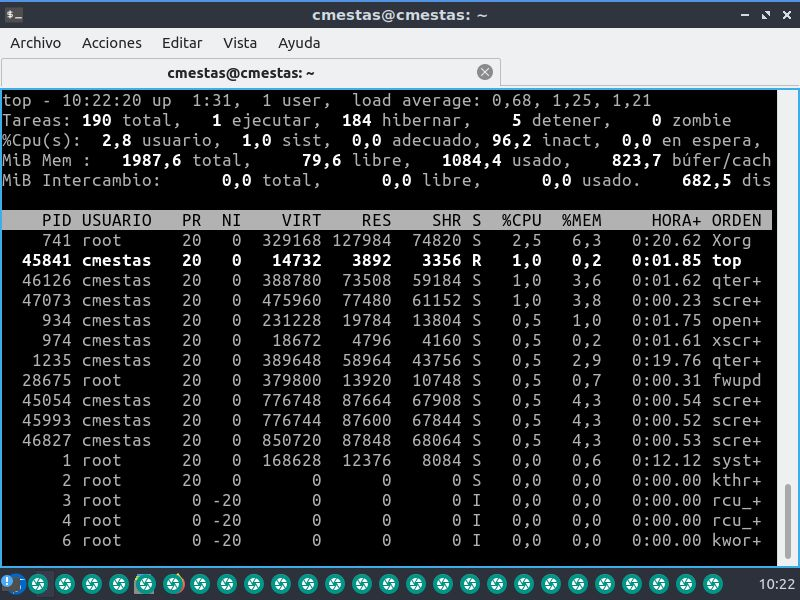
\includegraphics[width=0.65\textwidth]{images/screenA31.jpg}
    \caption{$top$ luego de la pausa}
\end{figure}

\begin{figure}[h]
    \centering
    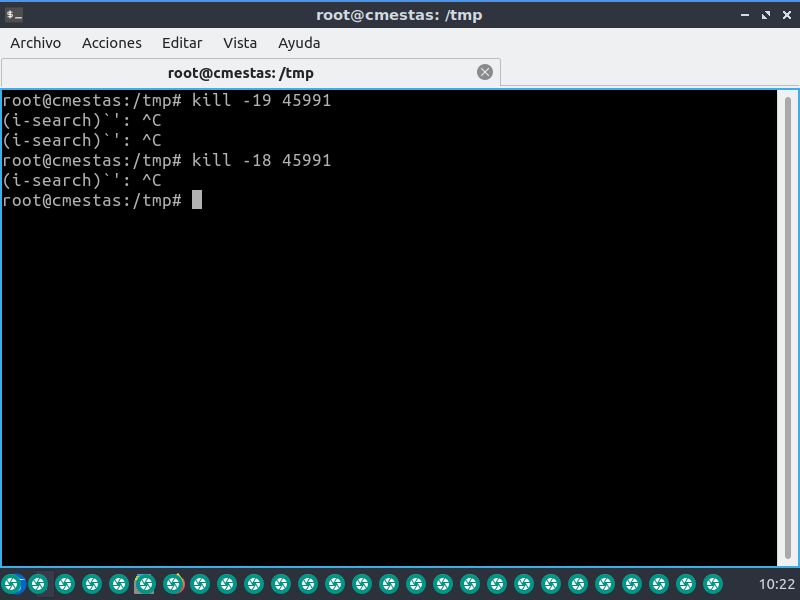
\includegraphics[width=0.65\textwidth]{images/screenA32.jpg}
    \caption{Reanudamos el bucle}
\end{figure}

\begin{figure}[h]
    \centering
    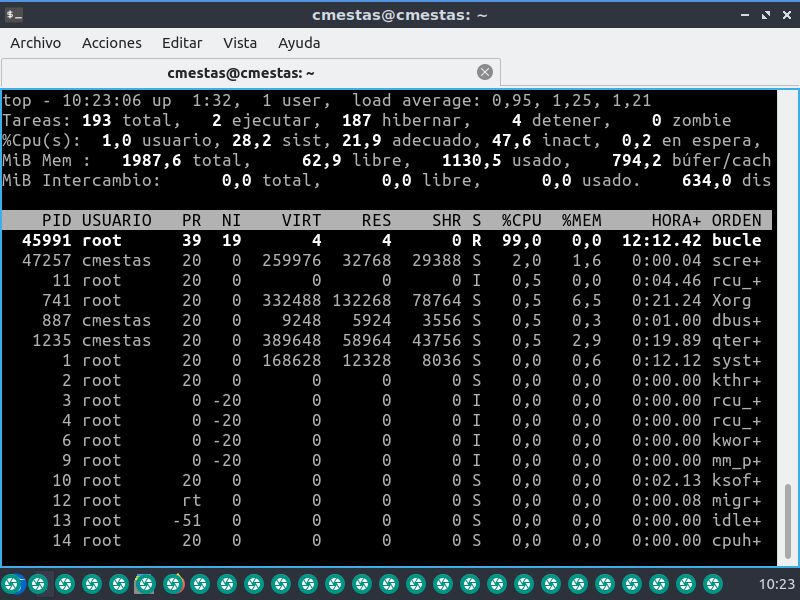
\includegraphics[width=0.65\textwidth]{images/screenA33.jpg}
    \caption{$top$ luego de reanudarlo}
\end{figure}

\begin{figure}[h]
    \centering
    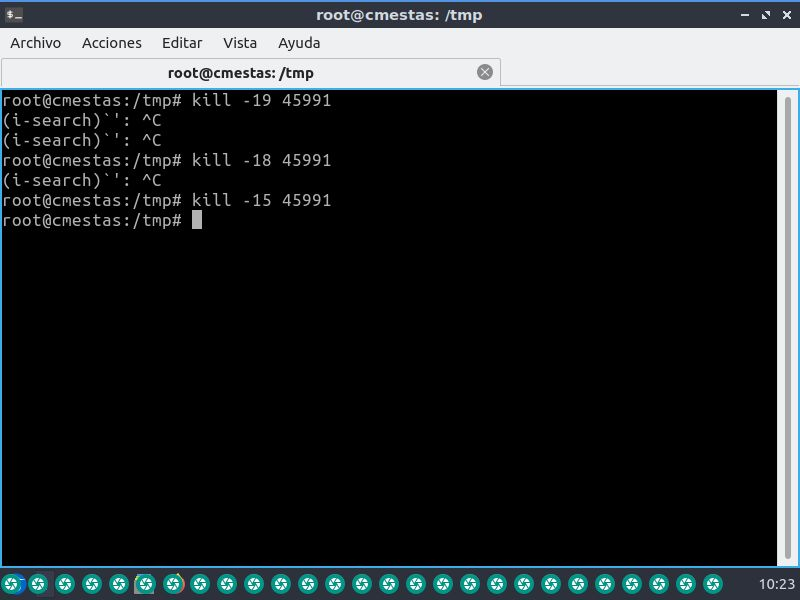
\includegraphics[width=0.65\textwidth]{images/screenA34.jpg}
    \caption{Eliminamos}
\end{figure}

\clearpage
\newpage

\begin{figure}[h]
    \centering
    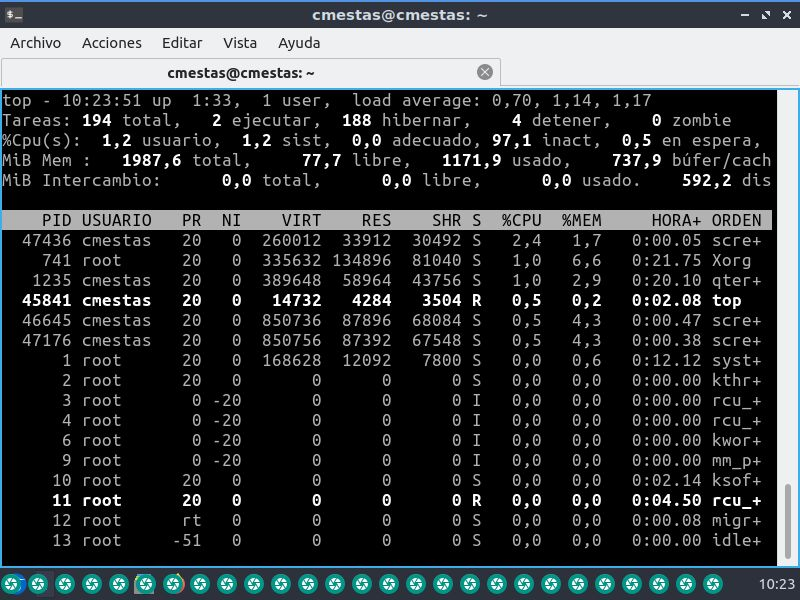
\includegraphics[width=0.65\textwidth]{images/screenA35.jpg}
    \caption{$top$ luego de eliminar}
\end{figure}

\begin{figure}[h]
    \centering
    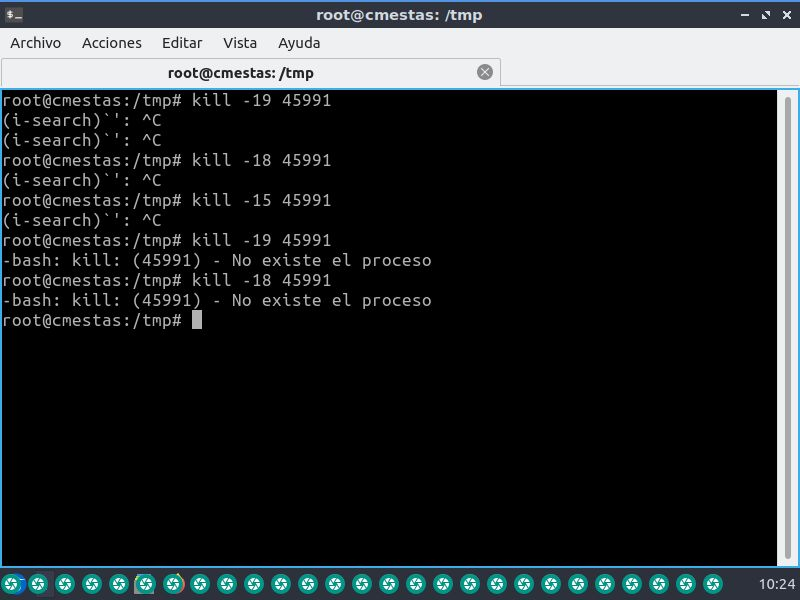
\includegraphics[width=0.65\textwidth]{images/screenA36.jpg}
    \caption{No se puede reanudar el proceso}
\end{figure}

Observamos que no podemos reanudar ni pausar el proceso porque fue eliminado anteriormente.




\end{document}


